%=============================================================================
% Background
% Copyright (c) 2018. Lester James V. Miranda
%
% This file is part of thesis-manuscript.
%
% thesis-mansucript is free software: you can redistribute it and/or modify
% it under the terms of the GNU General Public License as published by
% the Free Software Foundation, either version 3 of the License, or
% (at your option) any later version.
%
% thesis-manuscript is distributed in the hope that it will be useful,
% but WITHOUT ANY WARRANTY; without even the implied warranty of
% MERCHANTABILITY or FITNESS FOR A PARTICULAR PURPOSE.  See the
% GNU General Public License for more details.
%
% You should have received a copy of the GNU General Public License
% along with thesis-manuscript.  If not, see <http://www.gnu.org/licenses/>.
%
% Created by: Lester James V. Miranda <ljvmiranda@gmail.com>
%=============================================================================

\chapter{Background of the Study}
\label{BackgroundChapter}

\par In this chapter, we begin by looking into the problem of protein
function prediction in the lens of how protein data is usually represented
(Sec. \ref{ProteinFunctionPrediction}). Then, armed with the knowledge that
proteins can perform multiple functions at once, we will frame the protein
function prediction problem as a multilabel classification task (Sec.
\ref{MultilabelClassification}). We will argue that learning new
representations from data is vital to accomplish this task (Sec.
\ref{FeatureExtraction}), and at the same time introduce the autoencoder
neural network as basis for our methods. We then examine previous works that
have tackled this problem with a similar approach (Sec.
\ref{LiteratureReview}) and finally, express our research motivation and
hypotheses throughout this work (Sec. \ref{Motivation}).

\section{Protein Data Representation}
\label{ProteinFunctionPrediction}

Approaching the protein function prediction problem requires an
understanding of how protein data is often represented. We always
describe proteins in two ways: first by their (1) \textit{features} or
characteristics, and then by their (2) \textit{labels} or functional
categories.

\subsection{Protein features from high-throughput methods}

\par High-throughput sequencing techniques ushered in the emergence of
genomic big data (\cite{reuter2015high}). Scientists conducted various
experiments (e.g. DNA microarray, phylogenetic trees, etc.) to profile
protein sequences, resulting to huge amounts of structured data available for
use. These datasets facilitated protein function prediction, either it through
biochemical or computational means (\cite{eisenberg2000protein,
marcotte1999combined}). We will use two protein benchmarks,
Yeast and Genbase, derived from these experiments.

\par We define a \textit{protein feature set} as a matrix $\mathbf{X}$ where
each row is represented as a protein sample $i=1\dots N$ and each column as a
specific measurement $j=1/dots d$. Both Yeast and Genbase datasets were
formed from microarray gene expression data, with the former containing
phylogenetic profiles as additional information. Succintly, the raw feature
set is defined as $\mathbf{X} \in \mathbb{R}^{N \times d}$ where $N$ and $d$
is the number of protein samples and attributes respectively.

\par It is vital to spend some time emphasizing that noise is intrinsic to
high-throughput data (\cite{hong2013estimating}). A DNA microarray, for
example, is formed by probing unique regions of a gene in order to detect
expressions present in the tissue. Probing is sometimes conducted
heterogeneously, for ``different parts of the body, different [organisms], or
different phases of the cellular cycle'' (\cite{nguyen2009noise}). Each step
has the potential to introduce noise that may be detrimental to our task. To
a greater extent, extracting features from noisy data can compound its effect
and damage our classification model. Later on, we will discuss the denoising
autoencoder as a way to reduce the effect of noise from our raw features; but
first, let's look into what these features correspond to\textemdash a
protein's function.

\subsection{Protein functions}

\par Proteins perform a variety of functions to maintain our survival. They
can be seen in almost every facet of any biological process: cell
reproduction, signalling, metabolism, and etc. A single protein can perform
multiple functions at once, indicating a one-to-many relationship. Let's take
a protein sample (YAL041W) from baker's yeast (\cite{elisseeff2001kernel})
and inspect its array of functions:

\begin{figure}[!h]
  \centering
  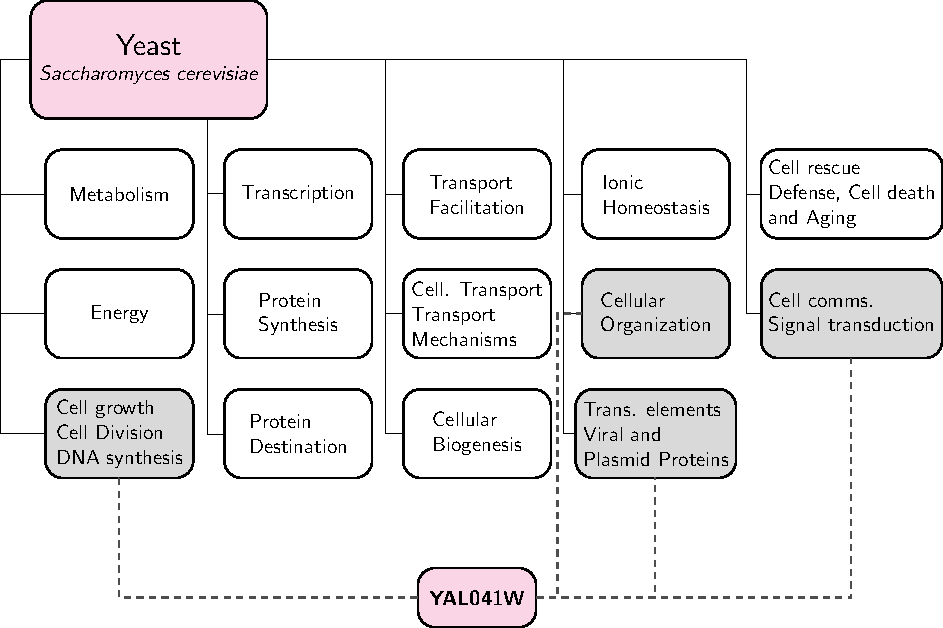
\includegraphics[width=0.75\textwidth]{ch01/demo_ontology}
  \caption{Functional categories of protein YAL041W in \textit{S. cerevisiae}}
  \label{demo:yeast_go}
\end{figure}

\noindent The protein above is associated with multiple functional
categories: cell growth, organization, communication, and viral detection. To
an extent, these categories are not necessarily related to one another yet
they are all performed by a single protein.

\par We define a set of protein functions (or \textit{labels}) as a binary
matrix $\mathbf{Y}$ where each row $i=1 \dots N$ is a protein sample, and
each column $j=1 \dots q$ is a protein function (designated as $\lambda$).
The size of $q$ depends on the number of possible labels in the dataset. In
addition, a protein labelset (a row vector) $\mathbf{y}_n$ is encoded as a
one-hot vector of size $q$. Say we're given a dataset with five functional
categories, $q=5$, and a protein sample $n$ that performs the functions
$\lambda_1, \lambda_4,$ and $\lambda_5$; we then express its labelset as:

\[
    \mathbf{y}_n = \left[\begin{matrix}
        1 & 0 & 0 & 1 & 1
    \end{matrix} \right]
\]

\noindent where each index indicates a protein's functional category. More formally, we
represent all protein labels as $\mathbf{Y} \in \{0,1\}^{N \times q}$, where each
row-vector $\mathbf{y}_n \in \{0,1\}^q$ is a labelset containing $q$ labels
$\lambda$.


\newpage
Together, we have the following definition:

\begin{definition}{}
A protein dataset $\mathcal{D}$ consists of $N$ pairs of feature and label
vectors $\{(\mathbf{x}_i, \mathbf{y}_i)\}_{i=1}^{N}$ where $\mathbf{x}_i \in
\mathbb{R}^d$ and $\mathbf{y}_i \in \{0,1\}^q$. In matrix-form, $\mathcal{D}$
consists of feature and label matrices, $\mathcal{D} = \langle \mathbf{X},
\mathbf{Y} \rangle$ where $\mathbf{X} \in \mathbb{R}^{N \times d}$ and
$\mathbf{Y} \in \{0,1\}^{N \times q}$.
\end{definition}

\par We will use this definition as we formulate the protein function
prediction problem as a multilabel classification task.


\section[Protein Function Prediction as a Multilabel Classification Task]
{Protein Function Prediction as a Multilabel\\Classification  (MLC) Task}
\label{MultilabelClassification}

\par Classification is one of the most common tasks in machine learning
(\cite{herrera2016multilabel}). Given input features $\mathbf{X}$ and its
corresponding label $y$, the goal is to find a mapping function $\mathcal{H}:
\mathbf{X} \rightarrow y$ that can accurately associate each set of
attributes to its particular label. For prediction, we formulate the mapping
function as $\mathcal{H}: \mathbf{X} \rightarrow \widehat{y}$. A good example
is image classification: given an image, we train a classifier to distinguish
what particular object it belongs to.

\begin{figure}[!h]
  \centering
  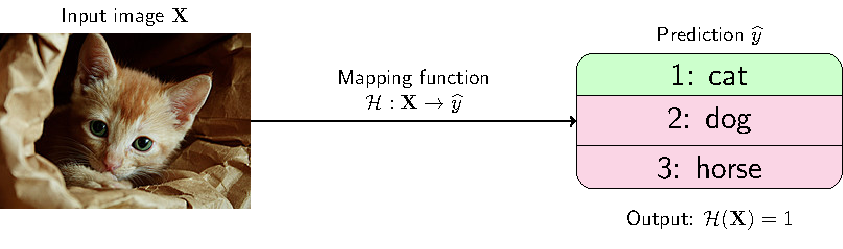
\includegraphics[width=0.70\textwidth]{ch01/demo_tradclass}
  \caption[Demonstration of traditional classification in images]
  {Demonstration of traditional classification in images.\\Cat photo
  from ImageNet (\cite{russakovsky2015imagenet})}
  \label{demo:traditional}
\end{figure}

\par However, proteins can perform multiple functions at once, and the
traditional definition of classification does not apply to the given task.
Instead, the goal now is to discriminate between \textit{multiple labels} and
associate them to the feature set. An apt counterpart to image classification
is scene classification (\cite{boutell2004learning}), where multiple objects
are associated to a given image.

\begin{figure}[!h]
  \centering
  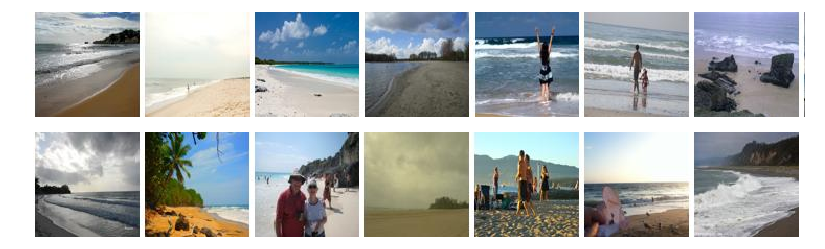
\includegraphics[width=0.95\textwidth]{ch01/demo_multilabel}
  \caption[Demonstration of multilabel classification]
  {Demonstration of multilabel classification.\\Beach photo
  from ImageNet (\cite{russakovsky2015imagenet})}
  \label{demo:multilabel}
\end{figure}

\newpage
\par Protein function prediction behaves similarly to scene classification:
given a protein sample (i.e., the image/scene), we are required to find the
functional categories associated with it (i.e., the objects in the scene).
This task is known as \textit{multilabel classification} (MLC). Notice that
in MLC, we only have two classes for each label $\lambda$: $0$ (does not
belong to $\lambda$) and $1$ (belongs to $\lambda$). Thus, MLC is akin to
doing binary classification for each label. Formally, we define the multilabel
classification task as:

\begin{definition}{}
Given a dataset $\mathcal{D}$, find a function $\mathcal{H}$ that maps the
feature matrix $\mathbf{X}$ to a set of labels $\mathbf{Y}$, i.e.,
$\mathcal{H}: \mathbf{X} \rightarrow \mathbf{Y}$. For any unseen instance
$\mathbf{x} \in \mathcal{X}$, where $\mathcal{X} \in \mathbb{R}^d$, we
predict its corresponding label vector $\mathbf{\widehat{y}}$ via
$\mathcal{H}(\mathbf{X}) \subseteq \mathcal{Y}$ where $\mathcal{Y} = \{y_1,
y_2, \dots, y_n, \dots, y_q\}$ and $y_n \in \{0,1\}$\footnote{Adapted from
\cite{zhang2014review}}.
\end{definition}

\par Next, we will discuss a commonly-used approach in solving multilabel
classification problems: binary relevance.

\subsection{Binary relevance in multilabel classification}

\par Binary relevance (BR) decomposes a multilabel problem into a series of
single-label classification tasks (\cite{godbole2004discriminative,
tsoumakas2007multilabel}). The concept is to take any ``off-the-shelf''
classifier $h$ and train it on each label $\lambda$, fitting a total of $q$
classifiers as seen in Figure \ref{demo:binaryrelevance}. Further
modifications to BR include combining labels, or building chains of
classifiers (\cite{read2009classifier}). However, due to BR's conceptual
simplicity and time-complexity\footnote[2]{
    Most problem-transformation techniques have an overhead time-complexity
    depending on the classifier $h$. For Binary relevance, we have $\bigO(q
    \cdot h(N, d))$. At inference, the complexity is $\bigO(q
    \cdot h(d))$. This is relatively faster compared to Classifier Chains
    $\bigO(q \cdot h(N, d + q))$ or Label Ranking $\bigO(q^{2} \cdot h(N, d))$
    (\cite{zhang2014review}).
}, it has been widely used in literature (\cite{zhang2017binary}).

\begin{figure}[!h]
  \centering
  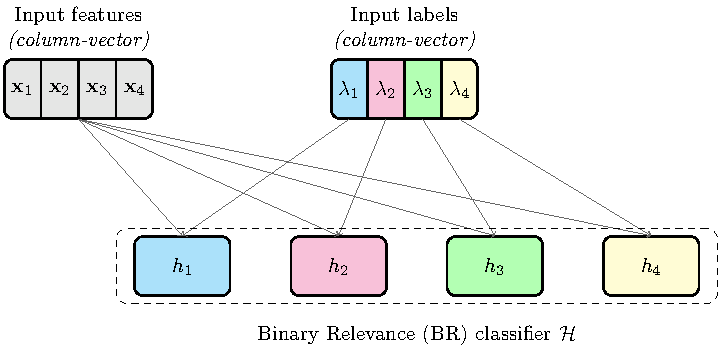
\includegraphics[width=0.65\textwidth]{ch01/demo_binaryrelevance}
  \caption[Binary relevance classification diagram]
  {Binary relevance classification diagram.\\Train $q$ classifiers $h$ for each
  label $\lambda$}
  \label{demo:binaryrelevance}
\end{figure}

\par BR falls under one of the two main approaches in classifying multilabel data:
problem transformation and algorithm adaptation. The former, where BR
belongs, transforms the multilabel problem into separate single-label binary
classification tasks while the latter adapts a classifier to directly handle
multilabel data (\cite{tsoumakas2007multilabel}).

\par We focus on BR for it is easier to treat the classifier as a separate
module from the feature extractor, and it is a simple yet effective method
for multilabel classification (\cite{luaces2012binary}). With BR, a
classifier can be decoupled from a feature extractor, enabling the former to
be tested on variants of the latter. Another reason is that the literature on
problem transformation techniques is extensive enough to enable benchmarking
of different multilabel classifiers in the future (\cite{zhang2014review,
madjarov2012extensive}).

\par This research will concentrate on finding good representations for the
BR classifier to solve the problem of protein function prediction. The
process of obtaining new features from raw data is called \textit{feature
extraction}, and is one of the core ideas in this work. Even if a BR
classifier can stand on its own, we hypothesize that higher performance can
be achieved with the extracted features than the raw data itself.

\section{Extracting Features for Better Data Representation}
\label{FeatureExtraction}

\par One of the core ideas in this work is feature extraction\footnote{
  Feature extraction has been referred to in various ways in literature:
  feature learning, representation learning, manifold learning, etc. We will
  use the term ``feature extraction'' in this work.
}\textemdash where new features are derived from raw attributes for better
data representation, and consequently, better classification. The success of
machine learning algorithms depends on data representations, for it can
entangle manifolds or explanatory factors of variation behind the data
(\cite{bengio2013representation}). 

\par More formally, the goal is to learn a mapping $\phi$ such that $\phi:
\mathbf{X} \rightarrow \mathbf{X}^{\prime}$, where $\mathbf{X}^{\prime}$
represents the extracted features useful\footnote{
  We will preemptively state that ensuring a feature set is useful will
  be the prime motivation of this work. We will attempt to define ``usefulness''
  or \textit{relevance} in Sec. \ref{Motivation}
} to a classifier $\mathcal{H}$. We
hypothesize that using $\mathbf{X}^{\prime}$ should provide better
classification (measured in accuracy, F-score, etc.) than just using the raw
attributes $\mathbf{X}$. The proceeding section will give a simple
demonstration using the XOR gate to illustrate this idea.

\subsection{A simple demonstration using the XOR gate}

\par Creating new features can be best illustrated with the XOR gate. The
goal is to separate binary 0's and 1's of the gate output. We take two
inputs $\mathbf{x} = \langle x_{1}$, $x_{2} \rangle, x_1, x_2 \in \{0,1\}$ as
features and its output $y_{i} \in \{0,1\}$ as the label. With $N=4$ samples
representing all possible bit-combinations, a dataset
$\mathcal{D}=\{(\mathbf{x}_{i}, y_{i})\}_{i=1}^{4}$ can be constructed as:

\[
    \mathcal{D} = \{(0,0,0), (0,1,1), (1,0,1), (1,1,0)\}
\]

Assuming we only have access to a linear classifier, the feature-space shown
in Figure \ref{demo:xor} (\textit{left}) proves that classifying the samples
is difficult due to its linear inseparability\textemdash that is, drawing a
single line to perfectly separate the X's and O's is impossible.
However, if a new feature-space $\mathbf{x}^{\prime}$ is engineered in such a
way that $\mathbf{x}^{\prime} = \langle {x}^{\prime}_{1}, {x}^{\prime}_2 \rangle$ where 
$x^{\prime}_{1} = \text{AND}(\bar{x}_{1}, x_{2})$ and $x^{\prime}_{2}
= \text{AND}(x_{1}, \bar{x}_{2})$, then it is possible to transform $\mathcal{D}$
into dataset $\mathcal{D}^{\prime}=\{(\mathbf{x}^{\prime}_{i}, y_{i})\}_{i=1}^{4}$
where:

\[
    \mathcal{D}^{\prime} = \{(0,0,0), (1,0,1), (0,1,1), (0,0,0)\}
\]

\par It can then be seen from Figure \ref{demo:xor} (\textit{right}) that
$\mathcal{D}^{\prime}$ is now a linearly separable problem. In this
demonstration, it is evident that hand-engineering features, or
\textit{extracting new features} has been helpful. However, with large
datasets, it will be tedious to manually find useful representations from
data. It is much preferable to automate the whole process. In the next
section, we will turn our attention to an effective way of learning $\phi$ in
a parameterized fashion\textemdash the autoencoder neural network.

\begin{figure}[!t]
  \centering
  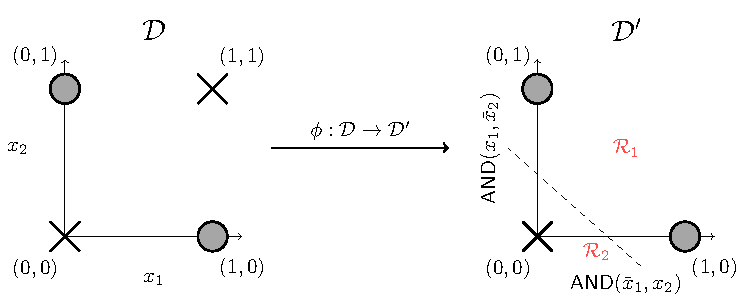
\includegraphics[width=0.75\textwidth]{ch01/demo_xor}
  \caption[Illustration of feature extraction using the XOR gate]
    {Illustration of feature extraction using the XOR gate.\\ Binary `1's are
    represented as circles while binary `0's as cross-marks.}
  \label{demo:xor}
\end{figure}

\subsection{The autoencoder neural network}

\begin{wrapfigure}{r}{0.5\textwidth}
  \centering
  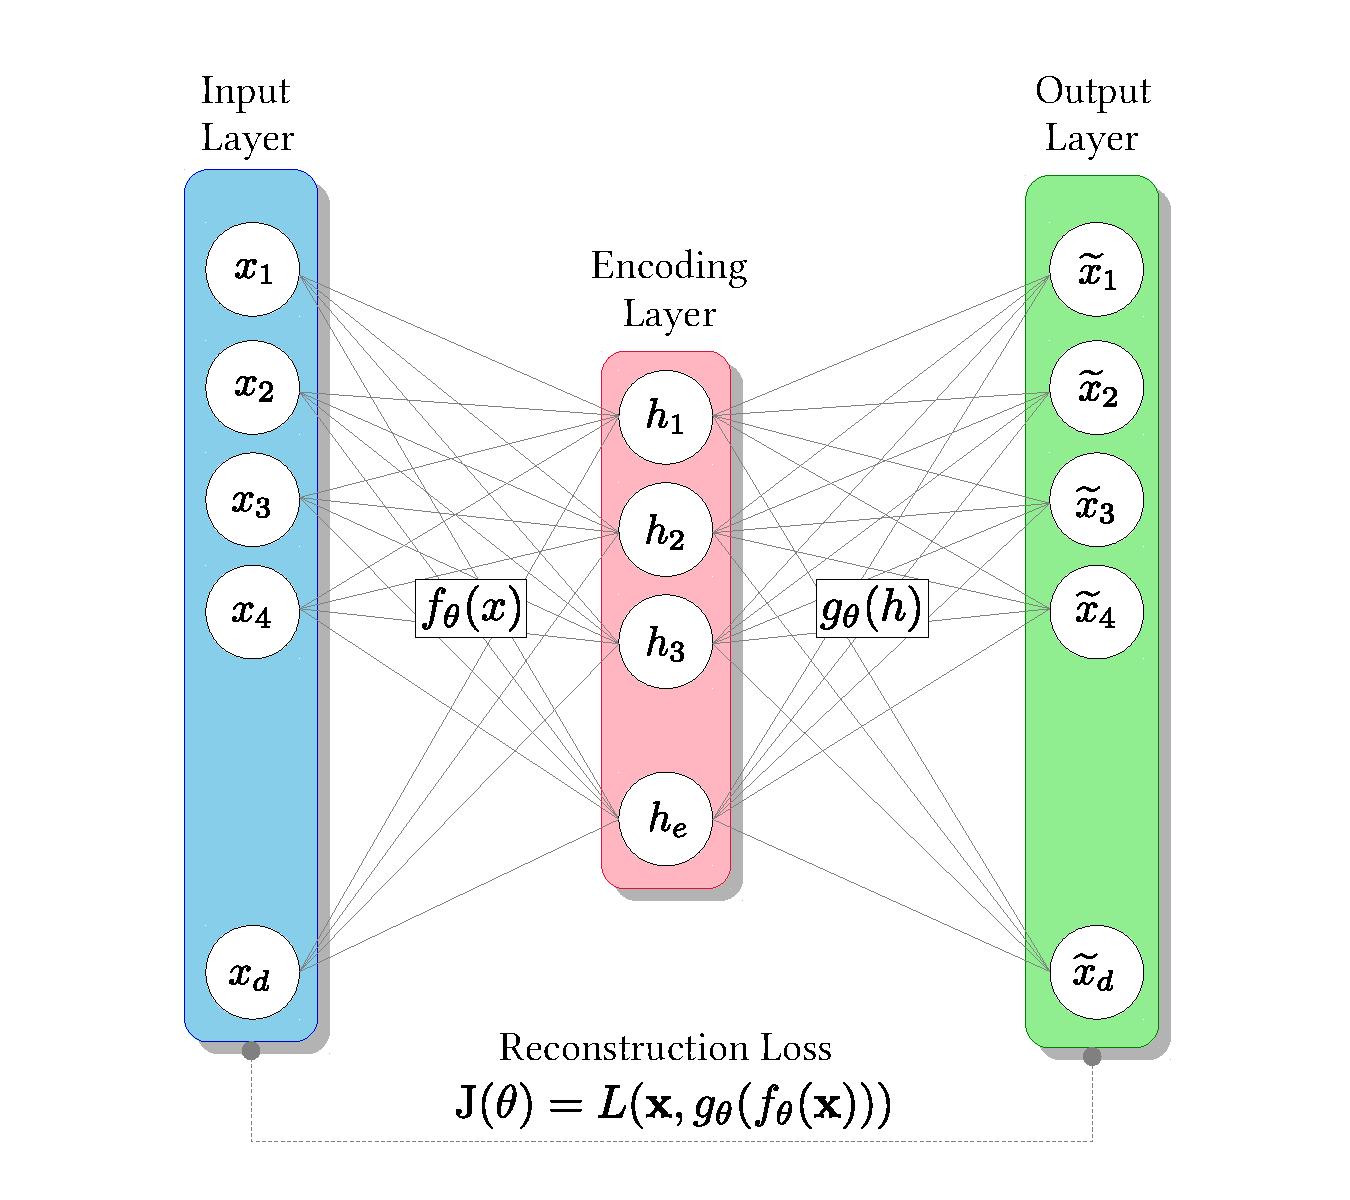
\includegraphics[width=0.40\textwidth]{ch01/schema_autoencoder}
  \caption[Diagram of the basic autoencoder]{
      Diagram of the basic autoencoder
  }
  \label{schema:autoencoder}
\end{wrapfigure}

\par This research is based on the autoencoder neural network as a framework
for solving the protein function prediction problem. It was first introduced
in 1987 (\cite{lecun1987phd}) and was subsequently studied in the following
years (\cite{bourlard1988auto, hinton1994autoencoders}). The idea is simple
yet powerful, that is, to have a network reconstruct a given input with the
presence of information bottlenecks.

\par There are two key aspects in training autoencoders: (1) information
reconstruction and (2) information bottleneck. The concept is that if an
autoencoder can reconstruct information ``perfectly'', even with constraints
involved, then it has learned the latent structure of the raw data. The
simplest way to constrain an autoencoder is by limiting the number of hidden
nodes $e$ less than the original dimension $d$ of the data. Say for example,
a dataset with $d=100$ dimensions. If we set $e=20$, and the autoencoder was
still able to reconstruct the original data ``perfectly'', then it has
learned a hidden structure from the data that was expressed in a lesser
capacity.

\par In practice, the autoencoder architecture consists of an encoder-decoder
scheme where the encoder function $f_{\theta}$ transforms the original input
$\mathbf{X}$ into a certain representation $\mathbf{h}$ (from $100$ features
to $20$), and the decoder function $g_{\theta^{\prime}}$ converts
$\mathbf{h}$ into an approximation of the raw features
$\mathbf{\widehat{X}}$ (where $\mathbf{\widehat{X}} =
g_{\theta^{\prime}}(\mathbf{h}) \approx \mathbf{X}$). Setting the loss
function as a comparison of the original input and its approximation
contrives the network to reconstruct $\mathbf{X}$:

\[
    J(\theta) = L(\mathbf{X}, \mathbf{\widehat{X}}) \quad \text{where} \quad
    \mathbf{\widehat{X}} = (g_{\theta^{\prime}} \circ f_{\theta}) (\mathbf{X})
\]

Algorithm \ref{algo:autoenc} describes the procedure for training an autoencoder.

%=============================================================================
% algo_autoenc.tex
% Copyright (c) 2018. Lester James V. Miranda
%
% This file is part of thesis-manuscript.
%
% thesis-mansucript is free software: you can redistribute it and/or modify
% it under the terms of the GNU General Public License as published by
% the Free Software Foundation, either version 3 of the License, or
% (at your option) any later version.
%
% thesis-manuscript is distributed in the hope that it will be useful,
% but WITHOUT ANY WARRANTY; without even the implied warranty of
% MERCHANTABILITY or FITNESS FOR A PARTICULAR PURPOSE.  See the
% GNU General Public License for more details.
%
% You should have received a copy of the GNU General Public License
% along with thesis-manuscript.  If not, see <http://www.gnu.org/licenses/>.
%
% Created by: Lester James V. Miranda <ljvmiranda@gmail.com>
%=============================================================================

\begin{algorithm}
    \caption{Training an autoencoder neural network}
    \label{algo:autoenc}
    \begin{algorithmic}[1]
    
    \INPUT Raw attributes $\mathbf{X}$
    \OUTPUT Learned parameters $\theta^{\ast}$

    \item[]
    \For{\textit{NumEpochs}}
        \State $\mathbf{h} \gets f_{\theta}(\mathbf{X}) = \sigma(\theta\mathbf{X}^{T} + \theta_0)$
        \Comment Encoder function
        \State $\mathbf{\widehat{X}} \gets g_{\theta^{\prime}}(\mathbf{h}) = \sigma(\theta^{\prime} \mathbf{h}^{T} + \theta^{\prime}_{0})$
        \Comment Decoder with tied-weights, $\theta^{\prime}=\theta^{T}$
        \State $J(\theta) \gets L(\mathbf{X}, \mathbf{\widehat{X}})$
        \Comment Compute loss
        \State \Call{Backpropagation}{$J(\theta)$}
        \Comment Optimize parameters
    \EndFor
    \State \Return $\theta^{\ast}$
    \Comment Return learned parameters
    \end{algorithmic}
\end{algorithm}

The learned parameters $\theta^{\ast}$ encapsulates the latent structure
discovered by the autoencoder. These parameters transform the original data
via the encoder function\textemdash i.e, $ \mathbf{X}^{\prime} =
f_{\theta^{\ast}}(\mathbf{X})$, $f_{\theta^{\ast}} \equiv \phi$\textemdash
and feed the transformation $\mathbf{X}^{\prime}$ into the multilabel
classifier $\mathcal{H}$. Figure \ref{schema:pipeline} illustrates this
simple model. In the next section, we will trace major developments in
machine learning that attempted to solve the protein function prediction
problem while adhering to the framework above.


\begin{figure}[!t]
  \centering
  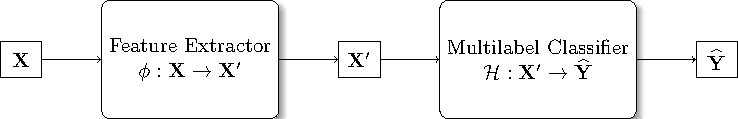
\includegraphics[width=0.85\textwidth]{ch01/schema_pipeline}
  \caption{Simple diagram of the protein function prediction model}
  \label{schema:pipeline}
\end{figure}

\section{Review of Related Literature}
\label{LiteratureReview}

\par There are three major movements we should consider when tracing the
developments of protein function prediction (PFP) in machine learning: first
is by (1) direct classification, then by (2) dimensionality reduction, and
lastly by (3) deep feature extraction. Machine learning techniques first
involved feeding raw data into a classifier, then found the need to reduce
the number of features in the dataset, and later on realized the importance
of learning suitable data representations for the classifier. This research
falls into the third category: utilizing deep neural networks to learn
representations for a multilabel classifier. But before that, let's start
from the beginning, where raw protein data is being fed directly to a
multilabel classifier.

\paragraph{Direct multilabel classification}
The earliest attempt to solve the protein function prediction problem was
done by \cite{elisseeff2001kernel}. They formulated PFP as a ranking problem
(not yet as a multilabel problem but rather an extension of multiclass
classification), and implemented a variant of the support-vector machine
(SVM) known as Rank-SVM. They tested their technique on \textit{S.
cerevisiae}, giving rise to the now known Yeast dataset. Later on,
\cite{diplaris2005protein} benchmarked various techniques on their own
protein data\textemdash the Genbase dataset. It is noteworthy that in the
conclusion of their work, they expressed their intention to investigate
``alternative representations of the learning problem,'' which brought a slew
of techniques for multilabel classification.

\par This brought forth the main baseline for multilabel classification, the
Binary Relevance (BR) algorithm
(\cite{godbole2004discriminative,tsoumakas2007multilabel}). These were then
extended into Label Powerset (LP) and Classifier Chains (CC)
(\cite{read2009classifier}), but BR's conceptual ease and ``relative speed''
enabled it to stay. Furthermore, various literature reviews attested BR's
performance, especially when paired with an SVM classifier
(\cite{luaces2012binary, zhang2014review,tsoumakas2017data}). For our
research, we will use the Binary Relevance with SVM (BR-SVM) as the baseline
of our work.

\paragraph{Reducing protein data dimensionality} Although binary relevance
has achieved good traction in protein function prediction, training a
classifier for each label can be time-consuming. Researchers have then
resorted to reduce the number of features in protein samples\footnote{The Genbase
dataset, for instance, has $1186$ attributes} using dimensionality-reduction
techniques (\cite{wang2009using, wang2013protein, wang2017protein}); they may
not reduce the number of labels to train their classifier upon, but they can
reduce the time it takes to train one. It is important to note that these
techniques gave a semblance of feature extraction: reducing dimensions in
data may be akin to finding a different representation of a feature space.
However, dimensionality-reduction is still limited primarily due to it being
linear with less capacity (\cite{cunningham2015linear}). Later on, we will
compare against the work of \cite{wang2013protein} that uses Principal
Component Analysis (PCA) as a dimensionality-reduction technique to a
k-nearest neighbors classifier (k-NN). They were able to reduce a protein
dataset with $353$ features into $204$, achieving good classification
performance. We chose this method because it follows a similar pipeline to
Figure \ref{schema:pipeline}, and uses a similar data source (gene
expressions) to our protein benchmark.

\paragraph{Deep feature extraction in protein function prediction}
Reducing dimensions in protein data has sped-up and improved classification,
but common approaches such as principal component analysis (PCA) are linear
(\cite{bengio2013representation}), failing to capture the nonlinearities
present in a protein's feature space. This gave way for researchers to apply
deep learning techniques to protein data\textemdash both for protein
sequences (\cite{bhola2014machine,kulmanov2017deepgo, zou2017protein}) and
expressions (\cite{baldi2001bioinformatics, chicco2014deep}). We
will benchmark against \cite{chicco2014deep}, who used a deep autoencoder
network to extract features from protein gene expressions. Comparing against
this method enables us to have a baseline, traditional autoencoder
implementation to check our proposed architecture upon.

\par As mentioned, our work falls under the last category of deep feature
extraction. One major advantage of this technique is that it can provide a
more separable feature space as demonstrated earlier by the XOR example. In
addition, we can decouple the feature extractor from the classifier with
binary relevance, enabling us to test on different variants of the
classifier. However, we argue that extracting features is not enough. It is
important to learn representations relevant with respect to the classifier.
The next section elaborates this work's motivation\textemdash clarifying the
meaning of feature relevance\textemdash and formulate the problem and
research hypothesis throughout this work.

\section{Research Motivation}
\label{Motivation}

\par Learning new representations from raw protein data has been effective in
capturing nonlinearities in the feature space\textemdash a feat unachievable
by dimensionality reduction or direct classification alone. However, there is
a need to ensure that the extracted features are indeed \textit{relevant}. It
is important to have useful representations, not just linear combination of
features and weights optimizing a loss function. Given these, we state our
reseasrch motivation:

% State the motivation of this work: it's not enough to extract features
% it is also important to extract relevant features.
\begin{quote}
  \itshape
  \small
  Although feature learning in protein data has been effective, we posit that
  merely extracting features is not enough. It is important to ensure that
  the extracted features are relevant with respect to the task at hand.
  Hence, we propose two autoencoder-based techniques to accomplish this task.
  Extracting relevant features should improve a classifier's predictive
  performance, bringing us a step closer to a faster and more efficient
  annotation of protein functions.
\end{quote}

\paragraph{Definitions of relevance}
Relevance depends on the question: ``relevant to what?''. Features must be
relevant with respect to (\cite{blum1997selection}):
\begin{itemize}
  \item the target concept (i.e. protein functions), and
  \item the task at hand (i.e., multilabel classification)
\end{itemize}

\par Various definitions of feature relevance exist depending on the
problem's goal. Because our main task is classification, we will adhere to
the definition of relevance as ``incrementally useful'':

\begin{definition}
  \label{DefRelevance}
   Given a dataset $\mathcal{D}$, a learning algorithm $\mathcal{H}$ and a
   feature set $\mathbf{X}$. A feature set $\mathbf{X}^{\prime}$ is
   incrementally useful to $\mathcal{H}$ with respect to $\mathbf{X}$ if the
   accuracy of the hypothesis that $\mathcal{L}$ produces using
   $\mathbf{X}^{\prime}$\footnote{Adapted from \cite{blum1997selection}}
   is better than the accuracy achieved using just the
   feature set $\mathbf{X}$.
\end{definition}

\par\noindent For multilabel classification, we will be using a different set
of metrics instead of accuracy. Originally, \cite{blum1997selection} uses
$\{x_{i}\} \cup \mathbf{X}$, but they went at length to extend this
definition to linear combinations of features, rather than just relevant
individual features. This validates the assumption that relevant features
should produce better predictions. In the next section, we will formulate the
problem and state our research hypothesis.

\subsection{Problem formulation and hypothesis}

\par The goal of this work is to extract a set of relevant features to
improve a classifier's performance in predicting protein functions. Formally,
the problem is defined as:

\begin{definition}
  \label{DefProblem}
  Given a dataset $\mathcal{D}=\langle \mathbf{X}, \mathbf{Y} \rangle$ and a
  classifier $\mathcal{H}$, construct a feature extractor $\phi$ that learns
  a feature set $\mathbf{X}^{\prime}$ by $\phi: \mathbf{X} \rightarrow
  \mathbf{X}^{\prime}$ such that $\mathbf{X}^{\prime}$ is relevant with respect
  to $\mathcal{H}$ and $\mathbf{X}$ by virtue of Def. \ref{DefRelevance}.
\end{definition}

\par\noindent We will explore two models that aims to accomplish this task.
Because these models extract task-relevant features, we expect that
classifier performance will improve. More formally, we state our research
hypothesis as:

\begin{definition}
  \label{DefHypothesis}
  If a feature extractor $\phi$ extracts task-relevant features
  $\mathbf{X}^{\prime\ast}$ for a multilabel classifier $\mathcal{H}$, then
  the performance of $\mathcal{H}(\mathbf{X}^{\prime\ast})$ should be
  better than the same classifier but with raw attributes $\mathbf{X}$
  or a non-relevant feature set $\mathbf{X}^{\prime}$.
\end{definition}


\par The next chapter (Ch. \ref{SDAEChapter}) will discuss the Stacked
Denoising Autoencoder (SdAE), examining its denoising capability to obtain
relevant features from an inherently noisy protein dataset. SdAEs were
originally used in image denoising, yet this work will explore its efficacy
in protein datasets in a multilabel setting. The following chapter (Ch.
\ref{SelectiveChapter}) will improve upon the autoencoder architecture via a
Mutually-Competitive autoencoder that learns a sparse and relevant feature
set by means of mutual competition. All resulting features from these models
will then be fed into a BR-SVM classifier. These autoencoder-based methods
will be tested with respect our hypothesis stated in Definition
\ref{DefHypothesis}.